\chapter{Hintergrund}
\label{cha:hintergrund}
Im Folgenden werden die Hauptbestandteile der Arbeit, die sich auch in deren Titel wiederfinden, näher erläutert. Dabei werden aus diesen Bereichen Paradigmen, Begrifflichkeiten und Funktionsweisen geklärt, die für das Grundverständnis der Masterarbeit notwendig sind. 

\section{Conversational User Interface}
\label{sec:conversational-user-interface}
Die Idee, mit Maschinen zu sprechen, gibt es schon lange. Bereits in den 1960er Jahren hat man mit textbasierten Dialog-Systemen angefangen, Konversationen zu simulieren. In den 1980er Jahren sind erste Sprachsteuerungen, bekannt als \acp{VUI}, auch kommerziell entwickelt worden. Hinzu gekommen sind in den 1990er Jahren die \textit{\ac{IVR}} Systeme, die es ermöglicht haben Sprache über das Telefon zu erkennen, um bestimmte Aufgaben zu erfüllen \cite{mctear-cui}. Noch heute findet man diese Systeme \zB bei Telefon Hotlines von DSL- und Mobilfunkanbietern. Häufig wird mit \ac{IVR} Systemen bei diesen Hotlines zunächst der Grund des Anrufs ermittelt und die Kundennummer abgefragt, um dann mit dem richtigen Ansprechpartner verbunden zu werden. \\
Bei der Interaktion mit diesen System sind Benutzer jedoch stark eingeschränkt. Die Eingabe Möglichkeiten belaufen sich lediglich auf strikt festgelegte, einzelne Befehle, Wörter und Phrasen. Aus diesem Grund wirken diese Dialoge eher unnatürlich und haben weniger mit Konversationen, wie man sie zwischen Menschen führt, zu tun. Des Weiteren durchläuft man einen festgelegten Konversationsfluss und hat keine Möglichkeit aus diesem auszubrechen.\\
Solchen Systemen beizubringen natürliche Sprache zu verstehen und Konversationen auf ähnliche Art und Weise wie Menschen zu führen, ist eine große Herausforderung. Hier gibt es viele Faktoren und Technologien, die dabei eine Rolle spielen.\\ 
Für das bessere Verständnis soll im Folgenden ein Überblick über diese Technologien, deren Bedeutung und Funktion gegeben werden. Diese Bereiche sind sehr komplex und beschäftigen Forscher seit Jahrzehnten. Es gibt zahlreiche Werke, die sich im Detail mit den genannten Themen auseinandersetzen. Entsprechende Verweise hierfür werden der jeweiligen Technologie hinzugefügt. Aus diesem Grund und da der Fokus der Arbeit ein anderer ist, werden sie nicht ausführlich beschrieben. 

\begin{itemize}
\item\textbf{\textit{\ac{AI}} oder \textit{\ac{KI}}}: Ein Gebiet, dass darauf abzielt, Maschinen an die Charakteristiken der menschlichen Intelligenz anzunähern. Da die Entwicklung noch nicht so weit geht, fällt das bisher Mögliche eher in den Bereich der \textit{Narrow AI}. Das bedeutet es sind Technologien, die bestimmte Aufgaben ähnlich gut oder sogar besser als Menschen bewältigen können. Typische Beispiele hierfür sind Klassifizierung von Daten, Gesichts-, Bild- und Sprach-Erkennung \cite{pereira-ai}\cite{copeland_difference_2016}. 
\item\textbf{\textit{\ac{ML}}}: Unter Verwendung von Algorithmen wird \ac{ML} zur Analyse von Daten verwendet. Auf Basis dessen können beispielsweise Entscheidungen getroffen oder Wahrscheinlichkeiten berechnet werden. \ac{ML} ist eine Herangehensweise, um künstliche Intelligenz zu realisieren \cite{camastra-ml}\cite{copeland_difference_2016}.
\item\textbf{\textit{\ac{ASR}}}: Mit Hilfe dieser Technologie kann ein Computer Worte, die eine Person in ein Mikrofon oder Telefon spricht in Echtzeit identifizieren und in lesbaren Text konvertieren. Häufig ist eine \ac{ASR} mit einer \ac{AI} \bzw mit \ac{ML} gekoppelt, um selbstständig dazu zu lernen. Dadurch kann die Genauigkeit erhöht werden, mit der Gesprochenes erkannt wird \cite{dong-asr}.
\item\textbf{\textit{\ac{NLP}}}: Mit Hilfe von \textit{\ac{NLP}} kann Text analysiert werden. Damit ist es beispielsweise möglich, Zusammenhänge innerhalb des Textes zu erkennen, die Semantik zu verstehen \bzw zu interpretieren und daraus Stimmungen zu erschließen \cite{biemann-nlp}. 
\item\textbf{\textit{\ac{TTS}}}: Wie der Name bereits sagt, wird ein \ac{TTS} System verwendet, um Text in Sprache zu konvertieren. Dabei können bereits aufgenommene Sprach-Artefakte zusammengesetzt oder auch menschliche Stimmen-Charakteristiken synthetisiert werden, um den Text als Audioausgabe zu generieren \cite{rao-tts}. 
\end{itemize}

Besonders die zunehmende Rechenleistung hat die Entwicklung dieser Bereiche in den letzten Jahren stark voran getrieben und sie nutzbar gemacht. Damit verbunden ist auch die Entstehung der jetzigen Generation von Dialog-Systemen, in Form von neuartigen \acp{VUI} und Chatbots. Angefangen mit der Veröffentlichung von Apple Siri im Jahr 2011, dem ersten kommerziellen Sprachassistenten der neuen Generation, sind bis heute weitere dazu gekommen. Dazu zählen \ua Microsoft Cortana\footnote{https://www.microsoft.com/en-us/windows/cortana, Abgerufen 31.10.2017}, Google Assistant\footnote{https://assistant.google.com, Abgerufen 31.10.2017} und Amazon Alexa. Abbildung \ref{fig:cui-funktionsweise} zeigt das typische Funktionsprinzip solcher \acp{VUI}.

\begin{figure}[!htb]
    \centering
    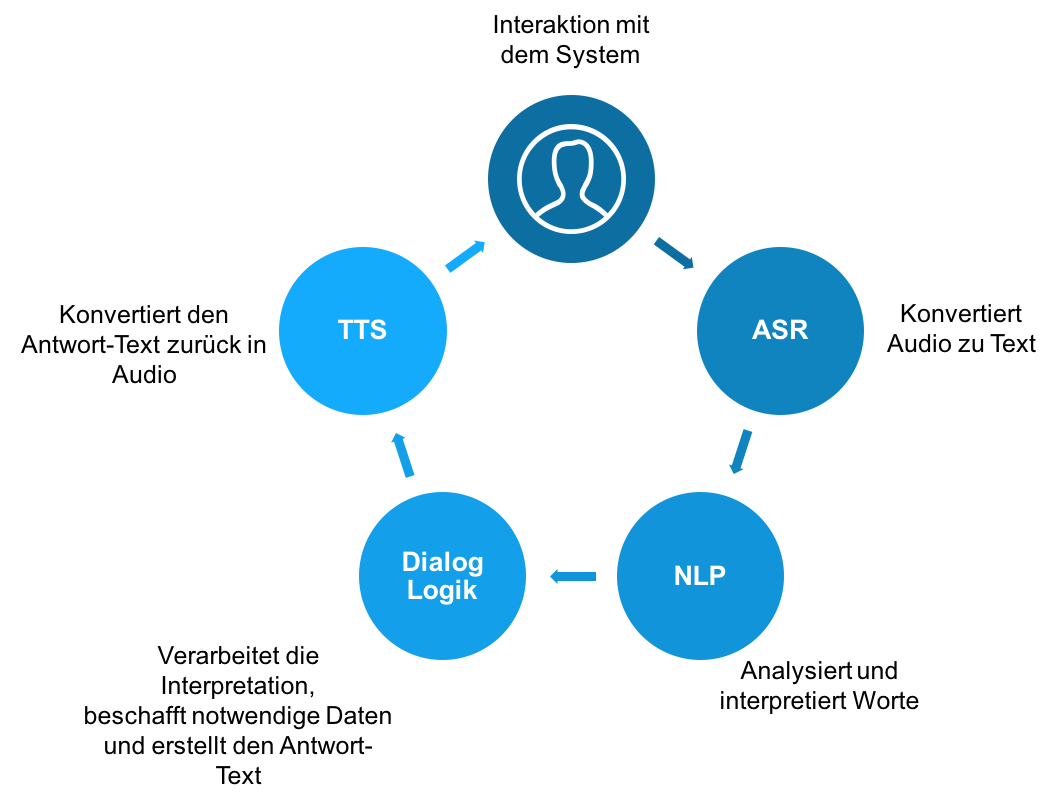
\includegraphics[width=\textwidth]{bilder/2_cuiFunktionsweise.png}
    \caption{Typische Komponenten und Funktionsweise eines VUI}
    \label{fig:cui-funktionsweise}
\end{figure}

Man kann diese \ac{VUI} Technologien an sich jedoch nicht als conversational bezeichnen. Dies soll anhand eines Beispiels von Amazon Alexa veranschaulicht werden, dass mit einer Konversation nicht viel zu tun hat.
 
\begin{center}
Nutzer: \textit{„Brauche ich heute in Nürnberg einen Regenschirm?“}\\
\textcolor{mybluelight}{Alexa: \textit{„In Nürnberg wird heute kein Regen erwartet.“}}\\
\end{center}

Alexa hat auch Anwendungsfälle, die mehr als eine einzelne Frage-Antwort-Interaktion erfordern. Den heutigen \acp{VUI} fehlt dennoch die Fähigkeit einen Schritt weiter zu gehen. Weg vom Kommandozeilen-Interface und hin zum \ac{CUI} \cite{pearl-design-vui}.

\begin{center}
\textit{„Many of today’s bots are kind of a hipster façade around the same basic command line interfaces consumers abandoned in the 1980s. They require specific syntaxes and understand only a limited vocabulary—but they sure have personality!“} \cite{hipster-facade-textio}
\end{center}

Konversation ist mehr als nur der Austausch von logischen Formulierungen. Verschiedene Handlungen wie zum Beispiel Fragen, Versprechungen und Komplimente finden statt \cite{mctear-cui}. Die Persönlichkeit der Konversationspartner hat einen großen Einfluss auf die Unterhaltung. Man stellt sich aufeinander ein und passt \ggf die Sprache an sein Gegenüber an. Ein weiterer Punkt ist der Kontext. Man kann sich im Verlauf einer Unterhaltung auf deren Vergangenheit beziehen. Im Folgenden ein Beispiel dazu. 

\begin{center} % so the minipage is centered
F: \textit{„Wer war Abraham Lincoln?“}\\
A: \textit{„Er war Präsident der Vereinigten Staaten.“}\\
F: \textit{„Wann hat er gelebt?“}\\
A: \textit{„Von 1809 bis 1865.“}\\    
\end{center}

Beim Stellen der zweiten Frage muss nicht explizit angegeben werden, wer gemeint ist. Dies wird aus dem Kontext heraus klar. Zusammengefasst lässt sich also sagen, dass folgende Kriterien ein typisches \ac{CUI} ausmachen: 
\begin{itemize}
    \item Ein Bewusstsein für den Kontext der Konversation
    
    \item Das Fehlen eines fixen Konversationsflusses und damit die Möglichkeit, den Kontext jederzeit zu wechseln
    
    \item Die Fähigkeit, den Benutzer nach kontextrelevanten Informationen zu fragen
    
    \item Persönlichkeit
\end{itemize}

Diese Art und Weise mit Schnittstellen zu kommunizieren bringt Vorteile mit sich. Wie in Kapitel \ref{sec:motivation} erwähnt, kann man einem \ac{CUI} die Frage stellen, anstatt sie über ein \ac{GUI} zu suchen. Das kommt auch Benutzern zu Gute, die mit der Bedienung grafischer Oberflächen Probleme haben. Es fällt ihnen möglicherweise leichter, ihr Vorhaben als Satz formuliert einzutippen \bzw in ein Gerät zu sprechen. Insbesondere \acp{VUI} eröffnen manch körperlich eingeschränkten Nutzern neue Wege der Interaktion mit Computern.\\
Das nächste Kapitel beschreibt das für die Arbeit verwendete System und geht auf dessen Funktionsweise ein. 

\section{Amazon Alexa Voice Service}
\label{sec:alexa-voice-service}
Amazon hat Alexa im November 2014 veröffentlicht. Wie bereits in Kapitel \ref{sec:conversational-user-interface} erwähnt, ist Alexa ein \ac{VUI} der neuen Generation. Es kann über die entsprechenden Endgeräte genutzt werden. Amazon hat zwei dieser Geräte zusammen mit Alexa veröffentlich. Die intelligenten Lautsprecher Echo \cite{amazon-echo} und Echo Dot \cite{amazon-echo-dot}, zu sehen in Abbildung \ref{fig:amazon-echos}. Mittlerweile sind weitere Ausführungen dazu gekommen. Für den weiteren Verlauf der Arbeit, wird als Vertreter aller Alexa Endgeräte ein Amazon Echo verwendet und schlicht als Echo, Alexa Endgerät oder Endgerät bezeichnet. Sämtliche Erläuterungen zur Funktionsweise und den Geräte-Merkmalen beziehen sich auf diesen.

\begin{figure}[h]
  \centering
  \begin{minipage}[b]{0.4\textwidth}
    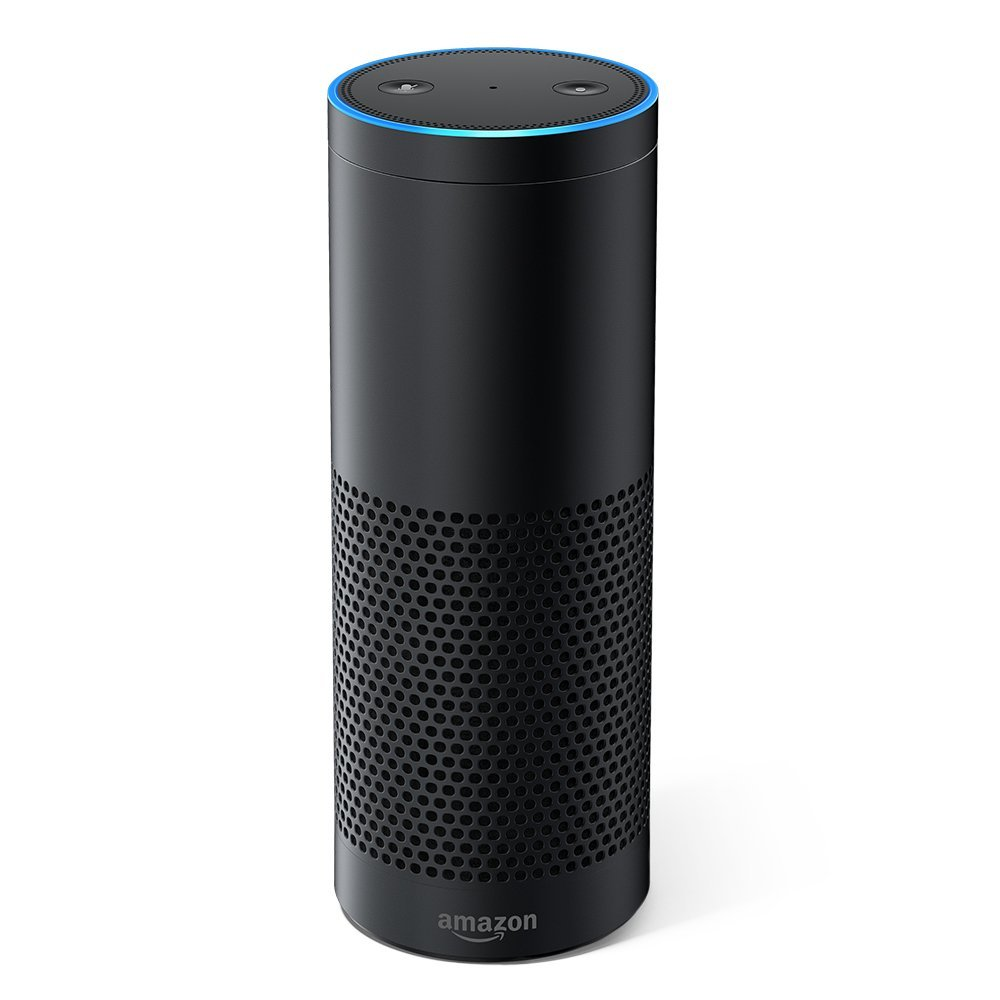
\includegraphics[width=\textwidth]{bilder/2_amazonEcho.jpg}
  \end{minipage}
  \begin{minipage}[b]{0.4\textwidth}
    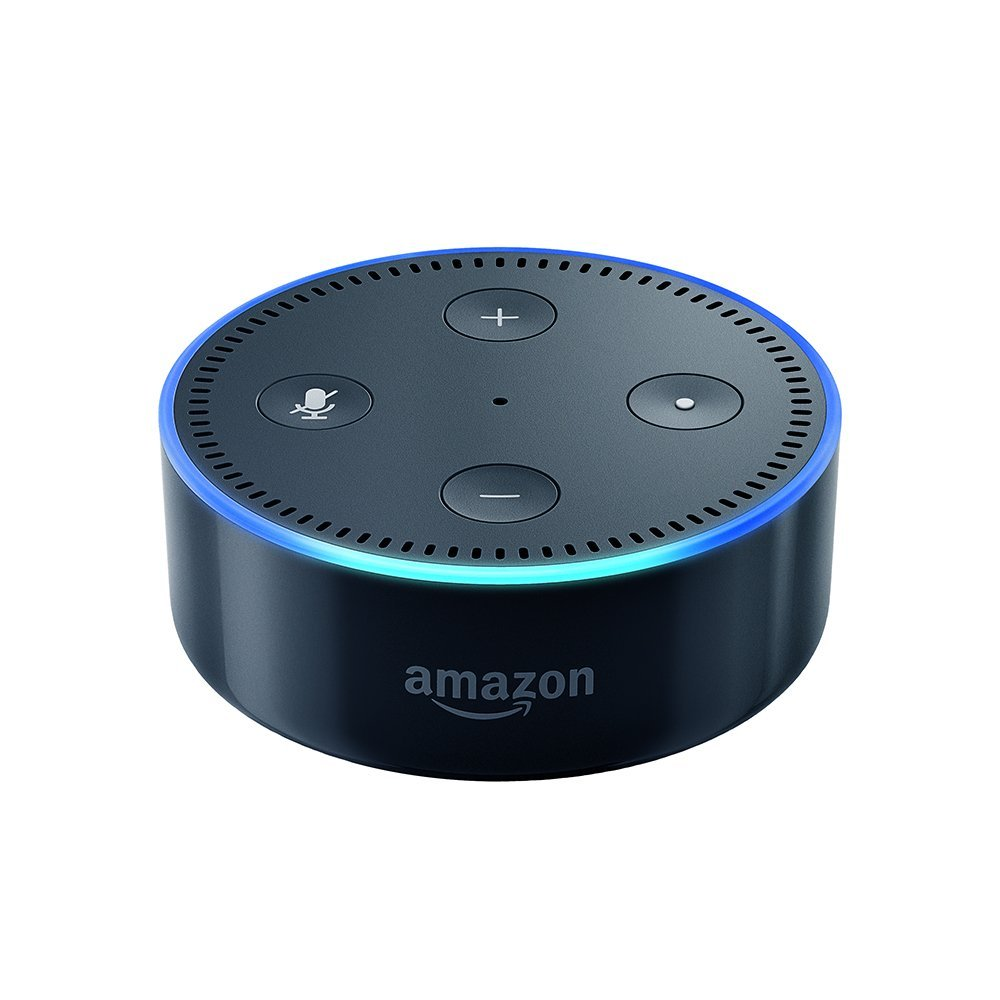
\includegraphics[width=\textwidth]{bilder/2_amazonEchoDot.jpg}
  \end{minipage}
  \caption{Amazon Echo und Echo Dot}
  \label{fig:amazon-echos}
\end{figure}

Die eigentliche Intelligenz steckt jedoch nicht im Echo. Alexa ist ein Cloud-Dienst \cite{amazon-developer-alexa}, der von Amazon über deren Server zur Verfügung gestellt und vom Endgerät genutzt wird (siehe Abbildung \ref{fig:alexa-komponenten}). 

\begin{figure}[!htb]
    \centering
    
\includegraphics[width=0.7\textwidth]{bilder/2_alexaDiagram.png}
    \caption{Alexa Endgerät zu Cloud-Dienst Verbindung}
    \label{fig:alexa-komponenten}
\end{figure}

Dabei bildet dieser Dienst einen Teil der \ac{VUI} Funktionalität ab und greift dabei auf die im Kapitel \ref{sec:conversational-user-interface} vorgestellten Technologien zurück. Um mit Alexa zu interagieren, muss ein Nutzer zunächst das sogenannte \textit{Wake Word} in den Echo sprechen. In der Grundeinstellung ist das Wort „Alexa“. Es kann jedoch auch auf „Echo“, „Amazon“ oder „Computer“ umgestellt werden. Mit einem Ton und dem leuchtenden Farbring auf der Oberseite des Echos signalisiert dieser, dass er sich mit dem Dienst verbunden hat und auf weitere Eingabe wartet. Nun kann man durch Sprache die gewünschten Funktionen nutzen. Der Lautsprecher kann sich nicht selbst aktivieren. Dies muss immer von einem Nutzer aus initiiert werden. \\
Alexa bringt bereits Basisfunktionalität mit, wie etwa Informationen zum Wetter, der Uhrzeit, das Verwalten von Timern und Listen und das Abspielen von Musik. Es ist jedoch auch möglich den Funktionsumfang durch zusätzliche Anwendungen, sogenannten Skills, zu erweitern. Um Skills zu nutzen die nicht in der Basisfunktionalität enthalten sind, muss man diese nach der Installation mit ihrem \textit{Invocation-Name} explizit ansprechen. In den meisten Fällen entspricht der Invocation-Name dem eigentlichen Namen des Skills. Es gibt zwei unterschiedliche Arten sie zu nutzen. Man kann sie öffnen und sich innerhalb der Anwendung bewegen, ohne den Namen wiederholen zu müssen. Die andere Möglichkeit ist das \textit{One-Shot-Model}. Hierüber wird der Skill beim Stellen der Frage direkt adressiert. Um beispielsweise die Anwendung „Abfallkalender“ \cite{abfallkalender} zu verwenden, welche Müllabfuhr Termine ausgeben kann, gibt es folgende Möglichkeiten. Öffnen des Skills: 

\begin{center} % so the minipage is centered
\textit{„Alexa, starte Abfallkalender“}\\
\textcolor{mybluelight}{Alexa: \textit{„Hallo hier ist der Abfallkalender, morgen am Montag wird Wertstofftonne abgeholt, kann ich sonst noch etwas für dich tun?}}
\end{center}
Nachdem der Abfallkalender geantwortet hat, kann man Fragen stellen wie: 

\begin{center} % so the minipage is centered
\textit{„Wann wird der Papiermüll abgeholt?“}\\
\textcolor{mybluelight}{Alexa: \textit{„Altpapier wird am Donnerstag dem 14. September abgeholt“}}
\end{center}

Das ergibt vor allem Sinn, wenn man mehrere Fragen an einen Skill hat. Über das One-Shot-Model kann man sich den Zwischenschritt sparen, wenn man nur eine einzige Information abrufen möchte.

\begin{center} % so the minipage is centered
Nutzer: \textit{„Alexa, frage Abfallkalender, wann der Papiermüll geholt wird?“}\\
\textcolor{mybluelight}{Alexa: \textit{„Altpapier wird am Donnerstag dem 14. September abgeholt“}}
\end{center}

Jeder mit einem Amazon Developer Account \cite{amazon-developer} kann Skills selbst entwickeln und Alexa Nutzern zur Verfügung stellen. Ein Skill besteht mindestens aus zwei Komponenten, dem \textit{Interaction Model} und dem \textit{Skill-Server}. 

\textbf{Interaction Model}\\
Man kann sagen, dass das Interaction Model aus \ac{VUI} Sicht das Frontend bildet. Hier gibt man Informationen wie den Namen des Skills, dessen Invocation-Name und die Adresse des Servers mit der Logik an (siehe Abschnitt Skill-Server). Obwohl beide meist identisch sind, dient der Name lediglich dessen Anzeige, während der Invocation-Name, die Worte für das Öffnen der Anwendung bestimmt. Des Weiteren wird im Interaction Model festgelegt, welche Formulierungen Alexa in Verbindung mit diesem Skill verstehen soll. Diese müssen in Form einer definierten Syntax angegeben werden. Die dabei verwendeten Begrifflichkeiten werden anhand eines Beispiels erklärt, wie man es bei der Verwendung des Wetter Skills finden kann.

\begin{center} % so the minipage is centered
\textit{„Alexa, \textcolor{mybluelight}{brauche ich \textcolor{red}{morgen} in \textcolor{red}{Nürnberg} einen Regenschirm?“}}
\end{center}

Da es sich bei dem Wetter Skill um eine Alexa Basisfunktionalität handelt, muss der Invocation-Name an dieser Stelle nicht genannt werden.\\

\textbf{\textit{Intent}}: Im Beispiel kann der Intent nicht direkt markiert werden. Er ergibt sich aus dem Verbund der Formulierung. Technisch gesehen ist es eine Funktion. Für den Wetter Skill könnte es beispielsweise einen Intent geben, der für alle Anfragen bezüglich des Niederschlags zuständig ist. Semantisch ist es die Essenz der Konversation oder auch die Absicht des Nutzers.\\

\textbf{\textit{Slot}}: Slots, im Beispiel \textcolor{red}{rot} markiert, sind eine Art Parameter. Unter Angabe von Slots haben Nutzer die Möglichkeit, ihre Anfragen zu parametrisieren \bzw zu spezifizieren. Im Beispiel sind \textit{\textcolor{red}{morgen}} und \textit{\textcolor{red}{Nürnberg}} Slots, die man durch andere Zeit- oder Ortsangaben ersetzen kann, \zB \textit{\textcolor{mybluelight}{„brauche ich am \textcolor{red}{10. Juni} in \textcolor{red}{New York} einen Regenschirm?“}}.\\

\textbf{\textit{Utterance}}: Eine Utterance, im Beispiel der Verbund aus blau und rot markiertem Text, ist eine Formulierung, die Slots enthalten kann. Über eine solche Formulierung wird ein Intent verwendet. Utterances werden explizit mit einem bestimmten Intent verknüpft. Ein Intent kann also von vielen Utterances angesprochen werden. Statt dem verwendeten Beispiel könnte man mit \textit{\textcolor{mybluelight}{„wird es \textcolor{red}{morgen} in \textcolor{red}{Nürnberg} regnen?“}} danach fragen.

\begin{figure}[!htb]
    \centering
    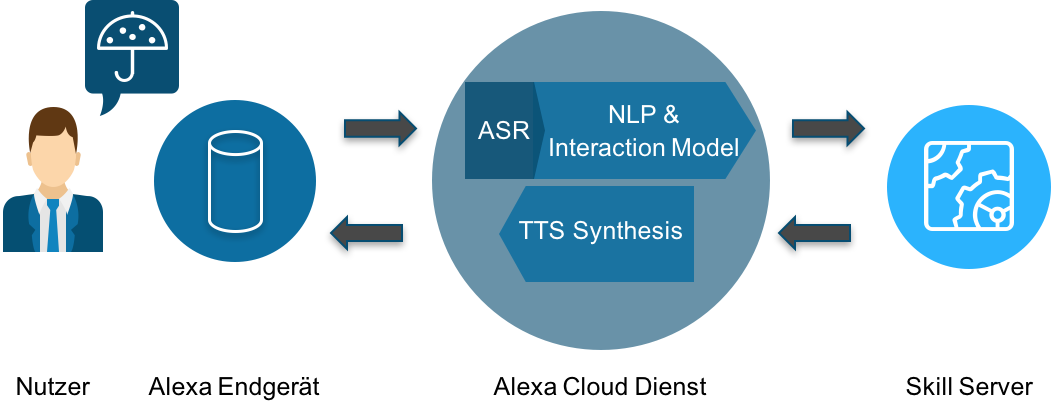
\includegraphics[width=0.7\textwidth]{bilder/2_alexaDiagramDetail.png}
    \caption{Alexa Komponenten und Funktionsweise}
    \label{fig:alexa-komponenten-funktionsweise}
\end{figure}

\textbf{Skill-Server}\\
Betrachtet man das Interaction Model als \ac{VUI}-Frontend, bildet der Skill-Server das Backend ab. Alexa sendet interpretierte Daten einer Spracheingabe über die im Model hinterlegte Adresse an die \textit{\ac{REST}}-Schnittstelle des Skill-Servers. Hier werden diese verarbeitet und  gegebenenfalls reale Daten entsprechend des Nutzungskontextes bereitgestellt. Die Antwort, die der Echo ausgeben soll, wird hier in Textform erstellt und an Alexa zurückgesandt. Das \ac{TTS} System aus Abbildung \ref{fig:alexa-komponenten-funktionsweise} konvertiert diesen Text in Audio. Im Anschluss wird das Audio an den Echo gesendet und von diesem ausgegeben. Es ist auch möglich grafische Elemente in die Interaktion einzubinden. Über sogenannte \textit{Skill Cards} kann man fest definierte, nicht veränderbare Strukturvorlagen mit statischem Text und Bildern erstellen. Diese kann der Benutzer über die Alexa Smartphone App auf seinem mobilen Gerät empfangen und einsehen. Da diese Vorlagen keine dynamischen Inhalte erlauben sind Anwendungsfälle, die auf komplexe, visuelle Elemente zurückgreifen müssen, wenig zweckdienlich. Beispiele hierfür sind detailreiche Statistiken, lange Listen und die Planung von Routen.

\section{Bankkonten-Management}
\label{sec:bankkonten-management}
Laut Statistiken aus dem Jahr 2017 (siehe \cite{online-bank-statista} \cite{online-bank-heise} \cite{online-bank-destatis}) verwendet in etwa jeder zweite in Deutschland Online-Banking. Das heißt sie erledigen ihre Bankgeschäfte bequem vom Rechner oder anderen Endgeräten aus. Kreditinstitute und Banken stellen hierfür ihren Kunden kostenlose Online-Portale und Anwendungen für mobile Endgeräte zur Verfügung. Mit Bankkonten-Management sind in dieser Arbeit einerseits Funktionen gemeint, die man überwiegend aus diesen Anwendungen kennt. Dazu zählen \ua die Anzeige des Kontostandes, das Durchführen von Überweisungen und die Einsicht der Umsätze. Darüber hinaus gibt es weitere Dienste, die mittlerweile auch von vielen Banken angeboten werden, jedoch meist aus modernen Finanzmanagement-Anwendungen von Drittanbietern bekannt sind. Beispiele hierfür ist der \textit{Finanzmanager} der Volksbanken Raiffeisenbanken \cite{vrbank-finanzmanager}, welcher auf Wunsch in das Online-Banking-Portal integriert werden kann oder die Smartphone-Applikation \textit{fymio} der TeamBank AG \cite{fymio}. Da Teile dieser Funktionalität und deren Begrifflichkeiten in Überlegungen und der Konzeption im weiteren Verlauf der Arbeit einfließen, werden diese kurz erläutert. Für die Arbeit werden sie in der hier beschriebenen Art und Weise verwendet und können von den Definitionen in den genannten Anwendungen Finanzmanager und fymio abweichen.

\textbf{\textit{Finanzperiode}}: Eine Finanzperiode beginnt mit dem Gehaltseingang und endet vor dem nächsten. \\
\textbf{\textit{Budget}}: Mit Budget ist in dieser Arbeit das bis zum Ende der Finanzperiode verfügbare Guthaben gemeint, dass sich aus Einnahmen und Fixkosten errechnet.\\
\textbf{\textit{Multibanking}}: Mit Multibanking ist die Möglichkeit gemeint, mehrere Konten verschiedener Banken und Kreditinstitute parallel an eine zentrale Anwendung anzubinden.\\
\textbf{\textit{Hauptkonto}}: Damit ist das Konto gemeint, auf das sämtliche Berechnungen und Aktionen angewandt werden. Auch wenn es möglich ist mehrere Konten anzubinden (\vgl Multibanking), muss eines davon als Hauptkonto selektiert werden. Möchte man beispielsweise vor der Durchführung einer Überweisung das Budget ausgeben lassen, wäre es irreführend, dies von allen Konten zusammen zu rechnen.\\
\textbf{\textit{Sparziel}}: Mit Sparzielen können Nutzer auf einem Sparkonto für einen beliebigen Zweck sparen. Dabei kann man je nach Wunsch einmalige oder regelmäßige Zahlungen an dieses Ziel übertragen. Als Teil des Sparkontos, existiert ein solches Ziel nur virtuell und nicht als eine Art separates Unterkonto.